\documentclass{article}
\usepackage{graphicx, caption, subcaption}
\usepackage{algorithm}
\usepackage{algpseudocode}
\usepackage{algorithmicx}
\usepackage{amsmath}
\usepackage{dirtytalk}


\usepackage{geometry}
\usepackage{float}

\usepackage{xcolor}


\title{Thesis AABL}
\author{Sander Kaatee}
\date{\today}

\begin{document}

\maketitle
\begin{abstract}
\noindent
Accelerated Argumentation-Based Learning (AABL) has shown significant improvements in accuracy and learning speed when compared to other state-of-the-art machine learning techniques. Despite its promising performance, the algorithm has certain limitations and potential for optimization. In this paper, we provide an in-depth analysis of the AABL algorithm, examine its limitations, and propose possible optimizations. We refactor the AABL algorithm to improve its readability and efficiency, while maintaining its overall performance. Our analysis reveals opportunities for further optimization of the AABL approach and offers insights into its applicability in various domains.
\end{abstract}

\section{Introduction}
The increasing complexity of artificial intelligence models presents a fundamental challenge. The lack of interpretability and transparency in these systems, i.e. their  'black box' nature, raises concerns about potential biases and discriminatory outcomes and hampers users' trust and acceptance of their decisions. Consequently, Explainable Artificial Intelligence (XAI) has emerged as a research area, seeking to bridge the gap between human comprehension and AI reasoning. This paper delves into one approach within the realm of XAI, namely Accelerated Argumentation-Based Learning (AABL), which combines the power of machine learning with the structured reasoning of argumentation to provide human-understandable explanations for AI decisions.
\\\\
AABL is an optimization of Argumentation-Based Learning (ABL), a machine learning (ML) technique that  outperforms state-of-the-art methods in terms of accuracy and learning speed \cite{ayoobi2019handling, ayoobi2021online, valk2020comparing}. Proposed by Ayoobi et al.\cite{ayoobi2021argue}, Both methods claim to be based on the Bipolar Argumentation Framework (BAF) \cite{amgoud2008bipolarity}, which in turn is an extension of the Abstract Argumentation Framework (AF) by Dung \cite{dung1995acceptability}.
\\\\
Although AABL has shown significant improvements over the original ABL process \cite{ayoobi2019handling}, there is a need to further investigate why this approach yields such promising results and explore its place in the machine learning/reinforcement learning literature. Additionally, for AABL we aim to assess the adaptability of AABL to other settings beyond its initial domain of application.
\\\\
 In this paper, we aim to address these research questions by providing a thorough examination of the AABL algorithm as proposed by Ayoobi et al. \cite{ayoobi2021argue}. We will begin by providing a background on AABL and an outline of the algorithm. We will then replicate the original results, after which we propose an optimization as a result of refactoring the original implementation of AABL. We will also make a comparison between AABL as it was implemented and AABL as it was described, we will look at the discrepancies between these two version in the discussion section of this paper. 
\\\\
The intention of this paper is to understand the AABL algorithm better and identify possible optimizations and shortcomings. By answering these research questions, our goal is to further optimize the AABL algorithm and deepen our understanding of its applicability in various domains.

\section{Background}
The original Argumentation Based Learning algorithm proposed by Ayoobi et al. in 2019 \cite{ayoobi2019handling} has made significant improvements in online incremental learning scenarios in comparison to other methods. The original ABL exhibited excellent performance with increased accuracy and learning speed. However, it was limited by its memory and computational efficiency \cite{ayoobi2021argue}. The authors addressed these limitations by introducing the AABL method, the pseudocode as given by Ayoobi et al. in \cite{ayoobi2021argue} is shown in section \ref{method2} as 'Algorithm \ref{alg:AABL}: Accelerated Argumentation-Based Learning'.
\\\\
The authors state that the Bipolar Argumentation Framework (BAF) \cite{amgoud2008bipolarity} is the basis of the AABL method \cite{ayoobi2021argue}. According to Dung \cite{dung1995acceptability}, an Abstract Argumentation Framework (AF) consists of a set of arguments and a binary relation that shows attacks between arguments. The BAF builds upon Dung's concept by incorporating the notion that some arguments may support a conclusion while others may oppose it. In Algorithm 1, the support relations are used to determine what recovery label the algorithm should use. The attack relations are added to the BAF graph in algorithm 2, note that in the provided pseudocode these attack relations are not accessed anywhere. 
\\\\
The purpose of the original ABL as presented in \cite{ayoobi2023fullthesis} is to provide a novel online incremental learning approach that can autonomously handle external failures resulting from changes in the environment. Existing research tends to offer special-purpose solutions, in \cite{ayoobi2023fullthesis} the authors claim that ABL generates a set of hypotheses that can "be used for finding the best recovery behavior at each failure state". Additionally, the authors claim that ABL addresses the issue of poor generalization observed in current online learning algorithms, making it applicable to various domains, including robotics. Moreover, as the approach is supposedly based on argumentation, it allows for generating an explainable set of rules suitable for human-robot interaction.

\section{Methods}
\label{methods}
We compare a total of three different algorithms: Accelerated Arugmentation Based Learning (AABL), Refactored Argumentation Based Learning (RABL), and our implementation of how AABL was described in the original paper \cite{ayoobi2023fullthesis} (table~\ref{tab:algorithms}).
\begin{table}[H]
\centering
\begin{tabular}{|l|l|l|}
\hline
\textbf{Name} & \textbf{Description}                                                                                            & \textbf{\begin{tabular}[c]{@{}l@{}}Detailed \\ description at\end{tabular}} \\ \hline
AABL          & \begin{tabular}[c]{@{}l@{}}Accelerated Argumentation Based Learning,\\ as implemented by H. Ayoobi\end{tabular} & Section~\ref{method0}                                                                     \\ \hline
RABL          & \begin{tabular}[c]{@{}l@{}}Our refactored version of the original\\ implementation of AABL\end{tabular}         & Section~\ref{method1}                                                                     \\ \hline
Pseudocode    & \begin{tabular}[c]{@{}l@{}}Our implementation of AABL\\ as it is described in\end{tabular}                      & Section~\ref{method2}                                                                     \\ \hline
\end{tabular}
\caption{The three algorithms compared in this paper}
\label{tab:algorithms}
\end{table}
\noindent
We test and compare the algorithms on the original scenarios as described by \cite{ayoobi2023fullthesis} (scenario 1, 2 and 3) in experiment 0, 1 and 2. In experiment 3 we compare all algorithms together on three newly described scenarios (i, ii, and iii). \\\\
In the original paper, AABL is tested by having to find solutions to an obstacle course. AABL is handed a state: a field consisting of 6 to 12 locations. The amount of locations depend on the scenario: for scenario 1 there are six locations, for scenario 2 there are nine and for scenario 3 there are twelve. For each location there can be an object consisting of a color and a concept (e.g. a blue ball or a yellow person). For each state there is one correct action associated, either: ask, push, alternative route or continue. Depending on the scenario there are only either one or two locations relevant for determining the correct action, the other locations/objects function as noise for the algorithm.
\begin{figure}[H]
    \begin{subfigure}[b]{0.55\textwidth}
        \centering
        \includegraphics[width=\textwidth]{scenario1.drawio.png}
        \caption*{Scenario 1}
    \end{subfigure}
    \begin{subfigure}[b]{0.55\textwidth}
        \centering
        \includegraphics[width=\textwidth]{scenario2.drawio.png}
        \caption*{Scenario 2}
    \end{subfigure}
    \begin{subfigure}[b]{0.55\textwidth}
        \includegraphics[width=\textwidth]{scenario3.drawio.png}
        \caption*{Scenario 3}
    \end{subfigure}
    \caption{The three original scenarios}
    \label{fig:scenarios123}
\end{figure}

Our three new scenarios are based on the original three scenarios. However, instead of the correct action being dependent on one or two locations, the correct action is dependent on whatever object is colored 'red'. Again the other locations/objects function as noise.

\begin{figure}[H]
    \begin{subfigure}[b]{0.55\textwidth}
        \centering
        \includegraphics[width=\textwidth]{scenarioi.drawio.png}
        \caption*{Scenario i}
    \end{subfigure}
    \begin{subfigure}[b]{0.55\textwidth}
        \centering
        \includegraphics[width=\textwidth]{scenarioii.drawio.png}
        \caption*{Scenario ii}
    \end{subfigure}
    \begin{subfigure}[b]{0.55\textwidth}
        \includegraphics[width=\textwidth]{scenarioiii.drawio.png}
        \caption*{Scenario iii}
    \end{subfigure}
    \caption{The three new scenarios}
    \label{fig:scenariosiii}
\end{figure}


\setcounter{subsection}{-1}
\subsection{Experiment 0: Replication}
\label{method0}
The original implementation of AABL is available on the author's GitHub page \cite{ayoobiGithub}. In this experiment we provide a replication of the author's original experiment as outlined in \cite{ayoobi2023fullthesis}. 
We will repeat the experiment described in \cite{ayoobi2023fullthesis} and use its original method for generating data as also provided on his GitHub \cite{ayoobiGithub}: we average 10 iterations of training on 200 scenarios on all three scenarios: scenario 1 (six locations, only one location relevant), scenario two (nine locations, two locations relevant) and scenario 3 (twelve locations, two locations relevant) (see figure~\ref{fig:scenarios123}).

\subsection{Experiment 1: RABL vs AABL}
\label{method1}
Ayoobi's original code, as taken from \cite{ayoobiGithub}, contains large amounts of unnecessary and unused code. Apart from that, the original code contains hard-coded optimizations such as automatic handling of empty locations.
\\\\
In response to these issues, we have performed a comprehensive refactoring of the code. We removed all unused functions and variables, and introduced variable names that conceptually align better with what the code is doing. We also changed certain types for more compact code while improving ease of understanding. Most importantly, we made a significant change to the algorithm.
\\\\
The original code calculated all possible subsets of features up to length L, even though it only used these subsets to determine location numbers. Therefore, we rewrote the algorithm to keep track of a list of locations instead. This change not only resulted in a more efficient algorithm but also significantly simplified the code, making it easier to understand and maintain. The pseudocode for the refactored AABL can be found at Algorithm \ref{alg:refactored}.
\\\\
We compared RABL against AABL \cite{ayoobiGithub} on scenario 1, 2 and 3 (see figure~\ref{fig:scenarios123}). We did 10 iterations of 200 steps using the original method for generating data as provided on GitHub \cite{ayoobiGithub}. 

\begin{algorithm}[H]
\caption{RABL}
\label{alg:refactored}
\begin{algorithmic}
\Procedure{Initialize}{scenario}
    \State possible\_location\_combinations $\gets \emptyset$
    \State recovery\_behaviors $\gets \emptyset$
    \State num\_features\_to\_consider $\gets 1$
    \State num\_of\_locations $\gets$ len(scenario)
    \State important\_locations $\gets \{0, 1, \dots ,$ num\_of\_locations $- 1\}$
\EndProcedure
\hline
\\\\
\Procedure{DetermineRelevantLocations}{all\_scenarios, recoveries}
    \State should\_change $\gets False$
    \If{len(all\_scenarios) $> 0$}
        \If{len(important\_locations) $> 0$}
            \Statex
            \Comment{Determine which combination of features and locations we must consider}
            \For {idx $\in$ important\_locations}
                \State numbers $\gets \{idx, idx + 1, \dots , idx + \text{num\_features\_to\_consider} - 1\}$
                \State selected\_loc\_with\_recov $\gets$ PrepareTable(all\_scenarios, recoveries, numbers)
                \State unique\_selected\_loc\_recov $\gets$ UniqueRows(selected\_loc\_with\_recov)
                \State unique\_selected\_loc $\gets$ UniqueRows(selected\_loc\_with\_recov[:,:-1])
                \State negative $\gets$ len(unique\_selected\_loc\_recov) - len(unique\_selected\_loc)
                \State UpdateImportantLocationsAndCombinations(negative, numbers)
            \EndFor
        \Else
            \State should\_change $\gets True$
            \State important\_locations $\gets \{0, 1, \dots , \text{num\_of\_locations} - 1\}$
        \EndIf
    \EndIf
    \Return should\_change
\EndProcedure
\hline
\\\\
\Procedure{Update}{best\_recovery, all\_scenarios, recoveries}
    \State AddRecoveryBehavior(best\_recovery)
    \If{DetermineRelevantLocations(all\_scenarios, recoveries)}
        \State num\_features\_to\_consider $\gets$ num\_features\_to\_consider + 1
    \EndIf
\EndProcedure
\hline
\\\\
\Procedure{MakeGuess}{current\_scenario, prev\_scenarios, prev\_recov}
    \If{possible\_location\_combinations is empty}
        \Return empty string
    \EndIf
    \State relevant\_locations $\gets$ first location combination in possible\_location\_combinations
    \State current\_objects $\gets$ the objects in relevant\_locations in current\_scenario
    \State recovery\_behavior\_weights $\gets$ Occurences of current\_objects-recovery\_behavior combination in all scenarios

    \State max\_behaviors $\gets$ recovery\_behaviors associated with max(recovery\_behavior\_weights)
    
    \If{len(max\_behaviors) == 1}
        \Return max\_behaviors[0]
    \Else{}
        \Return MostCommon(prev\_recov)
    \EndIf
\EndProcedure
\end{algorithmic}
\end{algorithm}


\subsection{Experiment 2: Pseudocode vs AABL}
\label{method2}
In chapter 3 of \cite{ayoobi2023fullthesis} the following pseudocode is provided for describing the AABL algorithm, see algorithm~\ref{alg:AABL}. An indepth description is presented in addition to this pseudocode. With this experiment we will compare these descriptions to the working of the original code, as provided on GitHub\cite{ayoobiGithub} and as was used to replicate the results of \cite{ayoobi2021argue} in experiment 0. In the discussion [TODO: appendix?] (section \ref{discussion}) we systematically go through the textual description as provided in  \cite{ayoobi2023fullthesis}, we provide literal quotations and then compare them to the pseudocode as well as the implementation as found on \cite{ayoobiGithub}.
\\\\
For this experiment we compared 'Pseudocode' against AABL \cite{ayoobiGithub} on scenario 1,2 and 3 (see figure~\ref{fig:scenarios123}). We did 10 iterations of 200 steps using the original method for generating data as provided on GitHub \cite{ayoobiGithub}

% \textit{TODO VRAAG: deze pseudocode's zijn geen letterlijke kopien van Ayoobi, maar zijn wel bedoelt als citaat. Wat is de correcte (niet-plagiaat) manier van deze pseudocode weergeven? }
\begin{algorithm}[H]
\caption{Accelerated Argumentation-Based Learning}
\label{alg:AABL}
\begin{algorithmic}[1]
\Require Current BAF graph, Data Instance $X$ entering the argumentation-based learning model, feature values subsets' length $L$, The class label or Best Recovery Behavior (BRB) for $X$
\Ensure The predicted label for $X$ called $Y$
\Procedure{Argumentation-Based-Learning}{$BAF$, $X$, $L$, $BRB$}
\State Extract all feature value combinations in $X$ with length $L$ and add them to a list called $Combs$.
\State Let $SNs$ be the set of supporting nodes (in form of “supporting-node $\rightarrow$ supported-node”) in the BAF.
\For{all $sn$ in $SNs$}
\For{all $comb$ in $Combs$}
\If{sn.supporting-node == comb}
\State $Y$.Add(sn.supported-node)
\EndIf
\EndFor
\EndFor
\If{$Y$ is not empty}
\If{Length($Y$) == 1}
\State Apply $Y$ to environment and observe the result.
\Else
\State Select a prediction in $Y$ at random ($Y$ := $Y[random\ index]$) and observe the result.
\EndIf
\Else
\State Randomly choose a prediction from the available class labels (observed recovery behaviors).
\State Increment $L$ := Update the BAF unit (using Algorithm 2 with input parameters: current BAF graph, BRB, Combs, SNs).
\EndIf
\While{(should Increment L == True)}
\State $L$ := $L+1$
\State Compute the combinations of the feature values again as $Combs$.
\State should Increment $L$ := Update the model with Algorithm 2.
\EndWhile
\State \textbf{return} $Y$
\EndProcedure
\end{algorithmic}
\end{algorithm}

\begin{algorithm}[H]
\caption{Updating the BAF Unit}
\label{alg:updateBAF}
\begin{algorithmic}[1]
\Require Current \textbf{BAF} graph, class label (\textbf{B}est \textbf{R}ecovery \textbf{B}ehavior)
\textbf{BRB}, Combinations of feature values for X called Combs, Set of Supporting Nodes in the BAF graph SNs
\Ensure A Boolean variable “should Increment L” that tells whether L needs to be incremented or not.
\State Let RNs be the set of all the class labels (Recovery behavior Nodes) in the BAF.
\State Let attacks be the set all the attack relations (for a $\in$ RNs and b $\in$ RNs the attack relations are in form of “a $\to$ b”) among the class labels (recovery behavior nodes) in the BAF.
\Statex
\Comment{Updating attack relations and class labels}
\If{BRB is not in BAF}
\State add BRB to the BAF graph;
\State add bidirectional attacks between BRB and all the other class labels (recovery behavior nodes) as follows:
\For{all rn in RNs}
\State attacks.add( BRB $\to$ rn )
\State attacks.add( rn $\to$ BRB )
\EndFor
\EndIf
\Statex
\Comment{Updating support relations}
\State Let should Increment L $:=$ True
\For{all comb in Combs}
\State Let Add Support $:=$ True
\For{all sn in SNs}
\If{sn.supporting-node $==$ comb}
\State Add Support $:=$ False
\If{sn.supported-node $\neq$ BRB}
\State Mark comb as a non-unique node that can not support any node in future.
\State Remove sn from the set supporting nodes in BAF SNs.
\EndIf
\EndIf
\EndFor
\If{comb is not Marked}
\State should Increment L $:=$ False
\EndIf
\If{Add Support $==$ True}
\State SNs.add(comb $\to$ BRB)
\EndIf
\EndFor
\State \textbf{return} should Increment L
\EndProcedure
\end{algorithmic}
\end{algorithm}
\subsection{Experiment 3: AABL vs RABL vs Pseudocode}
We compared all three algorithms described in Sections~\ref{method0},~\ref{method1} and~\ref{method2} together on the three new scenarios as described in Section~\ref{methods}. Instead of training on 200 instances for 10 iterations, we now train on 1000 instances for 10 iterations. 
\\\\
In addition to the three algorithms, we provide a reference level through a naive algorithm that always returns the most often seen correct recovery behavior. 


\section{Results}
\setcounter{subsection}{-1}
\subsection{Experiment 0: Replication}
\label{results0}
\begin{figure}[H]
    \centering
    \begin{subfigure}[b]{0.45\textwidth}
        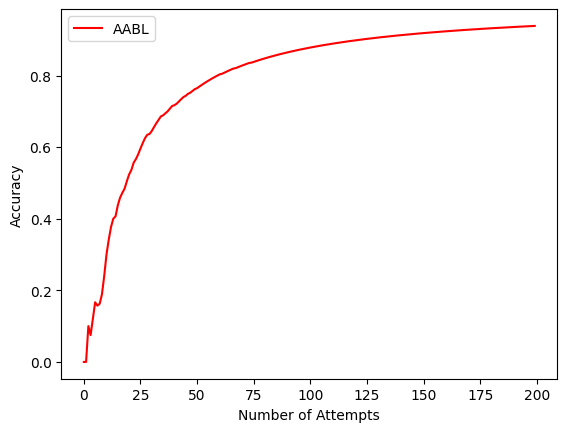
\includegraphics[width=\textwidth]{exp0_fig_first.png}
        \caption{Scenario 1}
    \end{subfigure}
    \begin{subfigure}[b]{0.45\textwidth}
        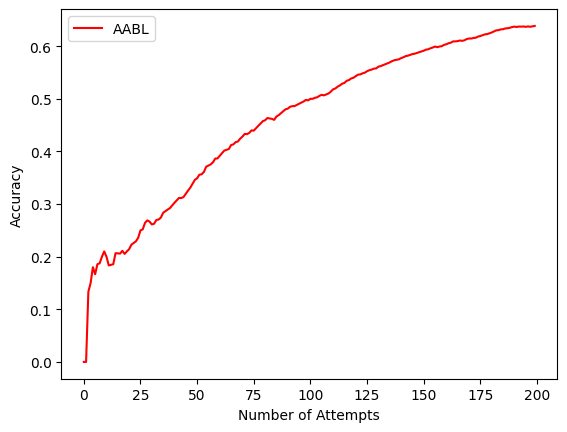
\includegraphics[width=\textwidth]{exp0_fig_second.png}
        \caption{Scenario 2}
    \end{subfigure}
    \begin{subfigure}[b]{0.45\textwidth}
        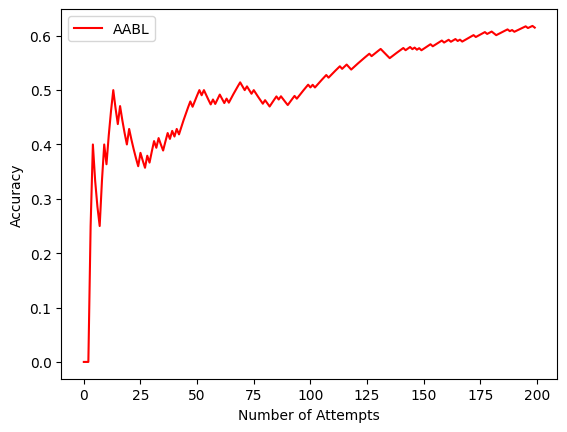
\includegraphics[width=\textwidth]{exp0_fig_third.png}
        \caption{Scenario 3}
    \end{subfigure}
    \caption{Performance of AABL taken from the author's Github\cite{ayoobiGithub}}
    \label{fig:exp0-results.png}
\end{figure}
\subsection{Experiment 1: RABL vs AABL}
\begin{figure}[H]
    \centering
    \begin{subfigure}[b]{0.45\textwidth}
        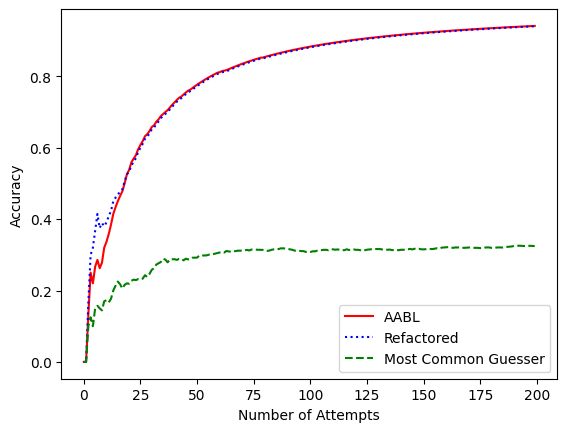
\includegraphics[width=\textwidth]{exp1_fig_first.png}
        \caption{Scenario 1}
    \end{subfigure}
    \begin{subfigure}[b]{0.45\textwidth}
        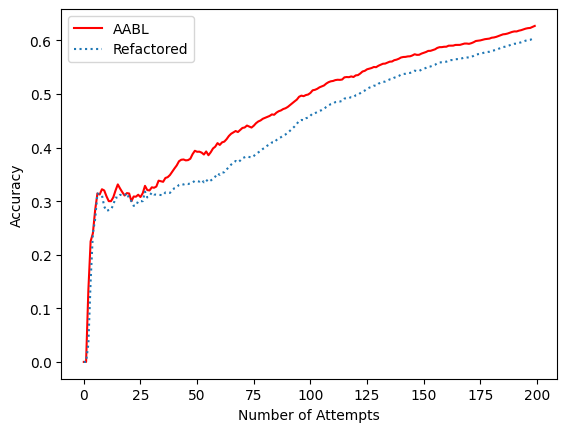
\includegraphics[width=\textwidth]{exp1_fig_second.png}
        \caption{Scenario 2}
    \end{subfigure}
    \begin{subfigure}[b]{0.45\textwidth}
        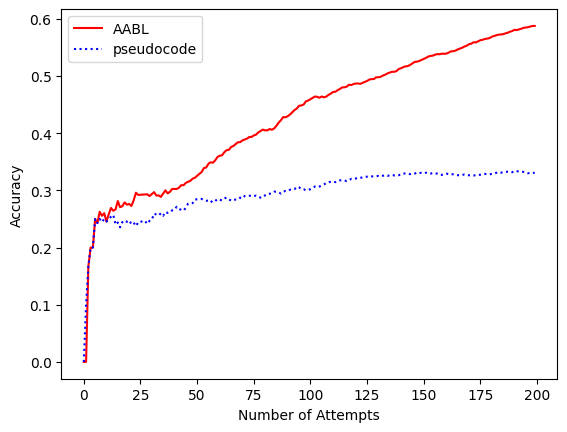
\includegraphics[width=\textwidth]{exp1_fig_third.png}
        \caption{Scenario 3}
    \end{subfigure}
    \caption{Performance AABL vs RABL}
    \label{fig:exp1-results.png}
\end{figure}
Figure \ref{fig:exp1-results.png} shows the comparison between the original implementation and the refactored version of AABL. When comparing the number of correct guesses at each of the 200 steps for 100 iterations, no significant difference was found between the two algorithms for the first two scenarios (for scenario 1: t = 1.4185, df = 39 998, p = 0.156, for scenario 2: t = -0.599, df = 39 998, p = 0.549). The refactored algorithm performs slightly better on the third scenario (for scenario 3: t = -2.123, df = 39 998, p = 0.033).
\\\\
These results show that the refactoring was indeed done correctly. In the graphs it is visible that for the first 5 - 30 scenarios the refactored algorithm slightly under-performs to the original AABL, however the provided t-test shows that this difference overal is not significant. The difference is most certainly due to the different implementation for determining the relevant locations, which causes the algorithm to be a bit slower with incrementing the number of features to consider.
\\\\
Although the slight and insignificant drop in performance in the first few guesses, the refactored algorithm performs quite a bit better in terms of compute time [TODO: and memory?] used, as shown in Table \ref{tab:refac-time-mem}.

\begin{table}[H]
\caption{Comparison of run-times for RABL and AABL.}
\label{tab:refac-time-mem}
\centering
\begin{tabular}{l|ll|}
\cline{2-3}
\textbf{}                             & \textbf{Time (seconds)}    & \textbf{} \\ \cline{2-3} 
                                      & \multicolumn{1}{l|}{AABL}  & RABL      \\ \hline
\multicolumn{1}{|l|}{First Scenario}  & \multicolumn{1}{l|}{2.09}  & 1.49      \\ \hline
\multicolumn{1}{|l|}{Second Scenario} & \multicolumn{1}{l|}{22.37} & 24.49     \\ \hline
\multicolumn{1}{|l|}{Third Scenario}  & \multicolumn{1}{l|}{74.47} & 85.22     \\ \hline
\end{tabular}
\end{table}


\subsection{Experiment 2: Pseudocode vs AABL}
\begin{figure}[H]
    \centering
    \begin{subfigure}[b]{0.45\textwidth}
        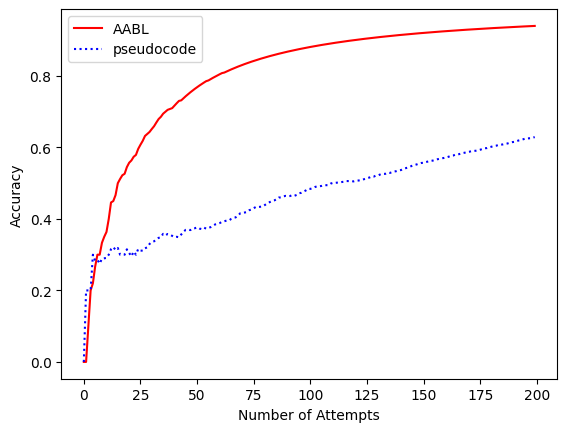
\includegraphics[width=\textwidth]{exp2_fig_first.png}
        \caption{Scenario 1}
    \end{subfigure}
    \begin{subfigure}[b]{0.45\textwidth}
        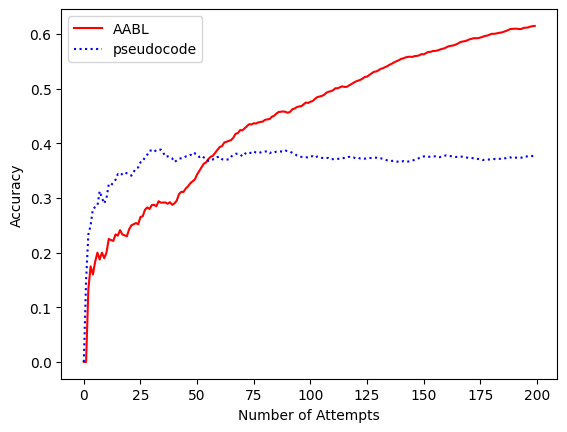
\includegraphics[width=\textwidth]{exp2_fig_second.png}
        \caption{Scenario 2}
    \end{subfigure}
    \begin{subfigure}[b]{0.45\textwidth}
        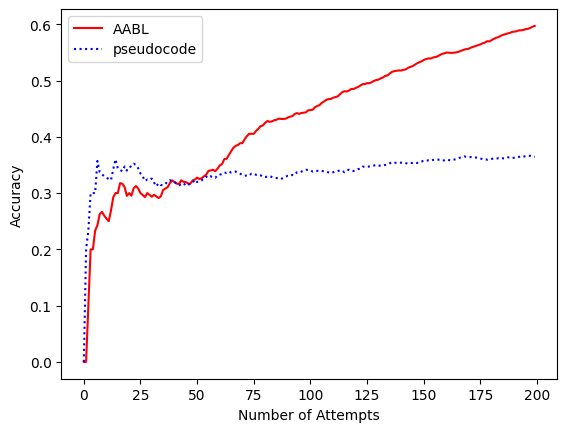
\includegraphics[width=\textwidth]{exp2_fig_third.png}
        \caption{Scenario 3}
    \end{subfigure}
    \caption{Performance of Pseudocode vs AABL}
    \label{fig:refactored-comparison.png}
\end{figure}
When comparing the accuracy at the 200th scenario, the results show that the re-implementation of the paper performed significantly worse than Ayoobi's AABL algorithm at accurately predicting correct recovery behaviors (for scenario 1: t = 15.98, df = 398, p $<$ 0.001, for scenario 2: t = 19.34, df = 398, p $<$ 0.001) 
% \subsection{Experiment 3: AABL vs Q-Learning}

\subsection{Experiment 3: AABL vs RABL vs Pseudocode}
\begin{figure}[H]
    \centering
    \begin{subfigure}[b]{0.45\textwidth}
        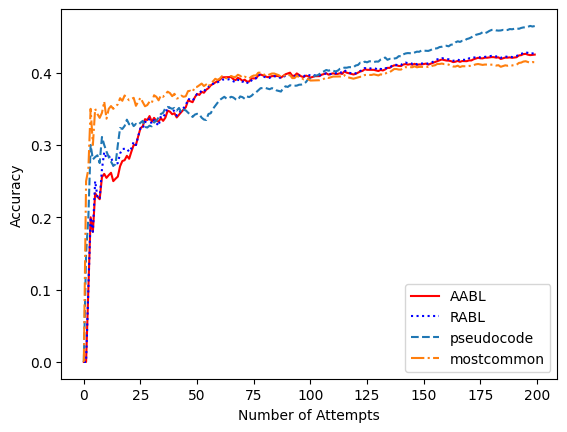
\includegraphics[width=\textwidth]{exp3_fig_first.png}
        \caption{Scenario i}
    \end{subfigure}
    \begin{subfigure}[b]{0.45\textwidth}
        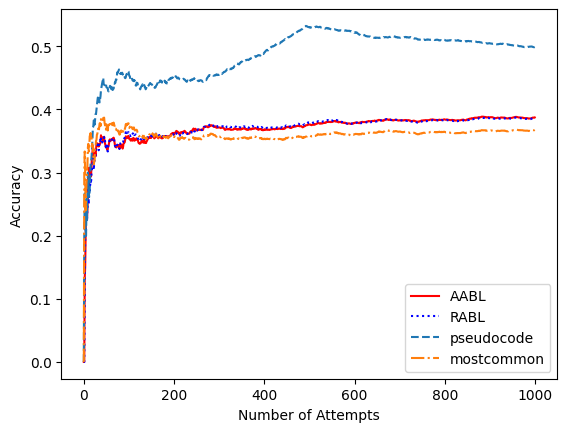
\includegraphics[width=\textwidth]{exp3_fig_second.png}
        \caption{Scenario ii}
    \end{subfigure}
    \begin{subfigure}[b]{0.45\textwidth}
        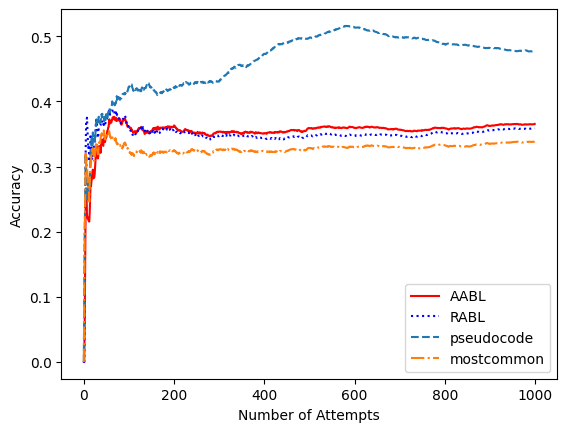
\includegraphics[width=\textwidth]{exp3_fig_third.png}
        \caption{Scenario iii}
    \end{subfigure}
    \caption{Performance of AABL vs RABL vs Pseudocode vs Most-Common on the newly described scenarios}
    \label{fig:exp3-.png}
\end{figure}

\newpage
\section{Discussion}
\label{discussion}
\subsection{Comparison of pseudocode, textual description and implementation}
In this subsection we will compare the three different forms of AABL that are available to us:
\begin{enumerate}
    \item \textbf{The textual description }- the description of what AABL does in words as given in 3.4.1 of chapter 3 of \cite{ayoobi2023fullthesis} "Explain what you see: argumentation-based learning and robotic vision" by Ayoobi
    \item \textbf{the pseudocode} - the description of what AABL does in pseudocode as given in 3.4.2 of chapter 3 of \cite{ayoobi2023fullthesis} "Explain what you see: argumentation-based learning and robotic vision" by Ayoobi
    \item \textbf{the original implementation }- AABL as implemented by Ayoobi taken from his GitHub \cite{ayoobiGithub}, which was used in Section \ref{method0} and \ref{results0} of this paper to verify the results as described in \cite{ayoobi2021argue}
\end{enumerate}
This section follows the linear example used in the textual description to compare these three versions of AABL. Since the workings of each version differ, we will sometimes need a tangent from the example in order to explain each method. \\\\
The example as given in 3.4.1 of chapter 3 of \cite{ayoobi2023fullthesis} is accompanied with the following table (\ref{tab:combinations}) and figure (\ref{fig:exampleofABL}), taken directly from \cite{ayoobi2023fullthesis}: 
\begin{table}[H]
\begin{center}
\caption{Possible combinations of color-type with the best recovery behaviors}
\label{tab:combinations}
\begin{tabular}{|c|c|c|c|}
\hline Order & Color & Concept & Best Recovery Behavior \\
\hline \hline 1 & Red & Ball & Push \\
\hline 2 & Red & Box & Alternative Route \\
\hline 3 & Red & Person & Ask \\
\hline 4 & Green & Ball & Push \\
\hline 5 & Green & Box & Alternative Route \\
\hline 6 & Green & Person & Ask \\
\hline 7 & Blue & Ball & Push \\
\hline 8 & Blue & Box & Alternative Route \\
\hline 9 & Blue & Person & Alternative Route \\
\hline 10 & Yellow & Ball & Push \\
\hline 11 & Yellow & Box & Alternative Route \\
\hline 12 & Yellow & Person & Ask \\
\hline 13 & None & None & Continue \\
\hline
\end{tabular}
\end{center}
\end{table}
\begin{figure}[H]
    \centering
    \begin{subfigure}[b]{\textwidth}
        \includegraphics[width=\textwidth]{screenshot.png}
        \caption{Scenario 1}
    \end{subfigure}
    \caption{Example of Argumentation-Based Learning for the illustrating
example}
    \label{fig:exampleofABL}
\end{figure}
\noindent
The figure (\ref{fig:exampleofABL}) supports the textual description as well as the pseudocode, as we shall see when walking through the textual description that the pseudocode and the textual description only differ in one aspect, namely: the pseudocode expects the correct answer to be handed as input while the textual description implies that AABL figures out the correct answer by trial and error. The original implementation does not correspond with the figure, as will become clear in the next section.

\subsubsection{Walk-through comparison}
The textual description in section 3.4.1 "Explanation of the Method with an 
Illustrating Example" from chapter 3 of \cite{ayoobi2023fullthesis} starts of with:
\begin{quote}
\textit{\say{
    We first use the simplified version of the test scenarios with only one location ahead of the agent (instead of 6, 9 or 12 locations). [...] the robot is initially confronted with a Red-Ball (R-Ba) and tries different recovery behaviors to find out that the best choice is Push.
}}
\end{quote}
However, in the pseudocode provided (Algorithm 1) we see that with an empty BAF graph the algorithm will reach line 18 and will randomly choose an observed recovery behavior. Since no recovery behavior has been observed yet, there will be no action. This corresponds with the original implementation: when the set of observed recovery behaviors is still empty, the original implementation immediately returns an empty string rather than trying out different recovery behaviors. Therefore on this point the pseudocode and implementation align while the textual description differs. 
\\\\
Instead of finding that the best choice is 'Push', the original implementation is handed the correct recovery behavior together with the confronted scenario. Although this differs from the textual description, it matches the pseudocode: Algorithm 1 requires as input the Best Recovery Behavior (BRB) for X. 
\begin{quote}
\textit{\say{
The model initially gets updated by the subsets of
feature values with size 1 (L := 1). This means that the supporting nodes R
and Ba are added to the Push recovery behavior
}}
\end{quote}
This aligns with the pseudocode, at line 19 a new algorithm (Algorithm 2) is called, which adds the features R and Ba as support relations to the 'Push' behavior. 
\\\\*
However, in the original implementation no such thing happens. There is no data structure that tracks support relations, instead the features are appended as $[0, red]$ and $[0, ball]$ to a list called \textit{subsets}, where 0 indicates the location of the object. 
\\\\
The recovery behavior 'Push' is uniquely added to a different list consisting of possible recovery behaviors. If the list of possible recovery behaviors were to already contain this recovery behavior then the recovery behavior is not added again: the original implementation does not track how often the recovery behavior is encountered. No relation between the subsets and recovery behaviors is tracked in any shape or form.
\\\\
Instead, the the original implementation will now try to determine a list of \textit{feature-locations} that could possibly be influencing the recovery behavior (In the original implementation the list of \textit{possible-feature-locations} is called "\textit{combination\_feature\_weights}", however we will refer to it as "\textit{possible-feature-locations}"). To determine these \textit{feature-locations} the algorithm requires as input a list of all previously encountered scenarios and the corresponding correct recovery behaviors. As the Red-Ball is the first scenario we encounter, this list is currently empty. Thus the list of \textit{possible-feature-locations} stays empty as well. In the next paragraphs we will take a deeper look at how \textit{possible-feature-locations} is updated and what the \textit{feature-locations} entail.

\begin{quote}
\textit{\say{
Subsequently, the agent encounters a Red-Box (R-Bo) for which the subsets of feature values with size L = 1 consist of R and Bo. Looking at the current state of the BAF, R supports the Push recovery behavior and it is chosen as the model’s
prediction.
}}
\end{quote}
This aligns with the pseudocode, at line 6 of Algorithm 1 the if-statement resolves to 'true' as '\textit{red==red}' and thus 'Push' would be added to the possibly correct responses Y. Then, at line 12 and 13, 'Push' is applied to the scenario as Y contains only one recovery behavior.
\\\\
In the original implementation there is no 'BAF' to look at, as the relations between 'Red', 'Ball' and 'Push' were not tracked. Instead the original implementation looks at the list of \textit{possible-feature-locations} that could be influencing the correct recovery behavior. Currently this list of \textit{possible-feature-locations} is empty.
\\\\
As the list of \textit{possible-feature-locations} is empty the algorithm again returns an empty string as recovery behavior. Thus on this point the original implementation again diverges from the pseudocode as well as the textual description. 

\begin{quote}
\textit{\say{
Since, this is a wrong choice, the agent try other recovery behaviors
and find “Alternative route” (Alt) as the best recovery behavior. Therefore,
the Alt node gets updated with its supporting nodes R and Bo and also a bidirectional attack among Alt and Push nodes. Since R supports both Push
and Alt recovery behaviors, it is not a unique supporter for each of them and
it will be pruned from both the recovery behaviors and will be marked as a
node which can no longer support any recovery behavior nodes in the future
}}
\end{quote}
As pointed out already, neither the pseudocode nor the original implementation try other recovery behaviors. However, the pseudocode does indeed update the 'Alt' node with the supporting nodes 'R' and 'Bo' at line 27 of Algorithm 2. Next to that, 'R' is indeed pruned and marked at line 18 and 19 of Algorithm 2. 
\\\\
The original implementation instead empties the list of subsets and appends \textit{[0, red]} and \textit{[0, box]} to the list of subsets, which now consists of \textit{[[0,red],[0,box]]} as \textit{[0,red]} and \textit{[0,ball]}, have been removed. 
\\\\
As the lists of previously encountered scenarios is now no longer empty, the algorithm will determine what \textit{possible-feature-locations} could be influencing the correct recovery behavior. The list of previous scenarios with their corresponding recovery behaviors currently only contains one scenario, namely: \textit{[Red, Ball, Push]} where Red is on column 0, Ball on column 1 and the recovery behavior on the last column. 
\\\\
We loop over each subset in \textit{subsets}. The first subset is \textit{[0, red]}, we take the location of this subset which is 0. When the subset contains a color we just keep the location as is, when it contains a concept we add 1 to the location. The algorithm will use these numbers to determine what column in the list of previous scenarios is important. In this case 0 corresponds with Red in \textit{[Red, Ball, Push]}. We then count the amount of unique occurrences of features in this column as well as the amount of unique occurrences of features in combination with recovery behaviors. If we find that there is a difference between these counts then we find that the recovery behavior does not correlate with this column and we discard the column. However as the list only contains one instance we find that there is no difference between the counts and thus we add the column to the list \textit{possible-feature-locations}, as it might be that this feature influences the correct recovery behavior.
\\\\
When a column is added to \textit{possible-feature-locations} a weight is calculated and added as well, the formula for this weight is: 
$$
weight = p + 1 + n * -50
$$
Where $p$ is the amount of non-unique feature-recovery occurrences
$$
p = TotalSelectedColumnsWithRecovery - TotalUniqueSelectedColumnsWithRecovery
$$
for this location and $n$ is the the amount of times this object appears in this location in combination with a different recovery behavior.
$$
n = TotalUniqueSelectedColumnsWithRecovery - TotalUniqueSelectedColumnsWithoutRecovery
$$
The only mention of weights in the description of AABL \cite{ayoobi2023fullthesis} claims that the weights are removed, namely the author states "\textit{ the
[total amount of] supporting weights and argument weights are reduced from 40 to 0.}". Thus there is no further explanation as to why this formula is chosen. 
\\\\
Note that we only add this weight in the case that there is \textbf{no difference} between the amount of unique occurrences of features in this column vs the amount of unique occurrences of features in combination with recovery behaviors, thus $n$ will always equal 0 when adding the weight. Which means that $$
weight = p + 1
$$
for every $feature-location$. 
\\\\
For \textit{[0, red]} the weight will be 0 as p equals zero since there is only one previously seen scenario (thus the the amount of unique feature-recovery pairs is equal to the total of feature-recovery pairs). 
\\\\
The same thing happens for the next subset \textit{[0, ball]}, as this subset contains a concept we look at column $location+1=1$. Again there is no difference between the amount of unique items in this column compared to the amount of unique 'items+recovery behaviors'. Thus we add column 1 to the list of \textit{possible-feature-locations} with a weight of 0 as well.
\begin{quote}
\textit{\say{
For the third learning instance the robot is confronted with a Red-Person
(R-P) and the models does not have any prediction since no current recovery
behavior node in the BAF has either P or R in its supporting nodes
}}
\end{quote}
This corresponds with the pseudocode as we saw in the previous paragraph that R was indeed pruned, next to that P has not been encountered yet. However for the original implementation, there is no BAF but instead we now have two entries in our list of \textit{possible-feature-locations}: column 0 and 1, corresponding to the color and concept of first object respectively. 
\\\\
The original implementation loops over these \textit{possible-feature-locations} and selects the first highest weight it encounters. Since both feature-locations in the list have equal weight, the algorithm selects the first column it encountered with the highest weight, which in this case is column 0. The algorithm then takes the feature associated with this location from the state, which is 'Red' as the current state contains \textit{[Red, Person]}. The algorithm then counts how often a recovery behavior is seen together with this feature in location 0. As we saw a Red-Ball and a Red-Box with recovery behaviors Push and Alt respectively, we get 1 for Push and 1 for Alt. If there is no single recovery behavior with the highest count, the algorithm instead returns the recovery behavior that has been most observed \textbf{overall}. As there's only been two observations: Push and Alt, the first one will be returned. Thus finally the algorithm wrongly predicts 'Push'.
\begin{quote}
\textit{\say{
The BAF unit gets updated with only P as a supporting node for the Ask since R
has been previously marked as a non-supporting node and bidirectional attack
relations are added among all pairs of the recovery behaviors
}}
\end{quote}
This aligns with the pseudocode. However, the original implementation instead will update the \textit{possible-feature-locations} which for now contains \textit{[0,1]} regarding column 0 and 1 respectively. 
\\\\
The list of subsets gets emptied and updated to \textit{[[0, Red],[0, Person]]}. The list of previously seen scenarios and their respective recovery behaviors will now be: $[[Red, Ball, Push],[Red, Box, Alt]]$.
\\\\
We loop over the subsets and start with $[0, Red]$, converting this instance to column 0. We then look in the previous scenarios and count the unique occurrences of features in this column: which is only 1, Red as this is the feature we saw in both previously seen scenarios. Then we count the amount of unique occurrences of features in combination with the respective recovery behaviors, which is 2 as Red occurs together with Push as well as Alt. Since these counts now differ, we remove column 0 from our list \textit{possible-feature-locations}. 
\\\\
The second subset \textit{[0, Person]} translates to column 1. We do the same counting and find two different features, namely \textit{Box} and \textit{Alt}. Since there is no difference between the amount of unique occurrences of features in this column vs the amount of unique occurrences of features in combination with recovery behaviors, this column stays in the list of \textit{possible-feature-locations} with a weight of 0, now being the only occurrence in this list. 
\begin{quote}
\textit{\say{
Subsequently, the agent encounters with a Green-Ball (G-Ba) obstacle and since Ba supports the Push in the BAF unit, Push is chosen as a prediction for the best recovery behavior.}}
\end{quote}
As the list of \textit{possible-feature-locations} only contains column 1, we take the feature associated with this column for this scenario, which is 'Ball'. We count the recovery behaviors associated with this feature as they are found in column 1 for all previously encountered scenarios. Since only the \textit{[Red, Ball, Push]} had the '\textit{Ball}' feature in column 1, '\textit{Push}' is correctly predicted as the best recovery behavior. 

\begin{quote}
\textit{\say{
The BAF gets updated using G supporting node for Push recovery behavior.
}}
\end{quote}
The list of subsets gets emptied and updated to \textit{[[0, Green],[0, Ball]]}. The list of previously seen scenarios and their respective recovery behaviors will now be: $$[[Red, Ball, Push],[Red, Box, Alt],[Red, Person, Ask]]$$
\\
We loop over the subsets and start with [0, Green], converting this instance to column 0. We then look in the previous scenarios and count the unique occurrences of features in this column: 1 as we so far have only encountered 'Red'. Then we count the amount of unique occurrences of features in combination with the respective recovery behaviors, which is 3 as Red occurs with 3 different recovery behaviors. Since both counts differ we do not add column 0 to our list of \textit{possible-feature-locations}. 
\\\\
The second subset is [0, Ball] which converts to column 1. The amount of unique occurences of features in this column is 3 as we so far have seen a 'Ball' a 'Box' and a 'Person'. The amount of unique occurences in combination with the respective recovery behavior is also 3 as each concepts occurs with a different recovery behavior. Since both counts are equal we add column 1 to our list of \textit{possible-feature-locations}. 
\\\\
We then calculate the weight for column 1, there are a total of 3 rows in the previous scenarios, each of which is unique thus the weight equals 0. [TODO: leg dit beter uit]



\begin{quote}
\textit{\say{
This process will continue and the model predicts the best recovery
behavior correctly in the subsequent obstacle confrontations until the agent
encounters a blue person.
When the agent encounters a Blue-Person (B-P), it chooses Ask as the
best recovery behavior. This is a reasonable choice because Ask was the best
recovery behavior for all the previous cases where a Person was the obstacle,
namely, in R-P and G-P. However, it turns out that the best choice for B-P
is Alt. Since, the subsets of feature values with size 1 were not adequate for
choosing the best recovery behavior for both the Ask and the Alt recovery
behaviors, the size of the subsets of the feature values is incremented i.e. L :=
L+1 in this case L = 2
}}
\end{quote}
[TODO]
\begin{quote}
\textit{\say{
Therefore, the supporting node B-P is added to the Alt
recovery behavior and the supporting nodes R-P and G-P are added to the Ask
recovery behavior while P is pruned and marked as a non-supportable node.
The model predicts the correct categories for the rest of the learning instances
until it is confronted with a Yellow-Person (Y-P). In this case the model does
not have any guess for the best recovery behavior and gets updated with the
Y-P supporting node.
}}
\end{quote}
[TODO]
\begin{quote}
\textit{\say{
The last learning instance None-None is a new case
based on the previous agent’s experiences and it does not have any prediction
for that. 
}}
\end{quote}
[TODO]

\begin{quote}
\textit{\say{
Finally the model gets updated and a new recovery behavior node
Continue (Cont) is added to the BAF model. In this illustrating example, the
proposed approach has seven correct predictions and two wrong predictions
out of all the thirteen instances while having no other predictions for the other
four cases. 
}}
\end{quote}
[TODO]
\begin{quote}
\textit{\say{
Notice that fixing the upper bound of L to 2 leads to good results in practice. This ensures the polynomial complexity of the resulting approach. 
}}
\end{quote}
[TODO]
\subsection{Summary}
\begin{table}[H]
\begin{center}
\caption{Difference between algorithms}
\label{tab:comparison}
\begin{tabular}{|l|l|l|l|}
\hline
                                      & AABL     & RABL     & Pseudocode \\ \hline
Support relations                     & Implicit & Implicit & Explicit   \\ \hline
Attack relations                      & Implicit & Implicit & Explicit   \\ \hline
Weights                               & Yes      & Yes      & No         \\ \hline
Subsets of features                   & Yes      & No       & Yes        \\ \hline
Hardcoded handling of empty locations & Yes      & No       & No         \\ \hline
\end{tabular}
\end{center}
\end{table}

\subsection{Analysis}
\subsubsection{Is It Argumentation Based}
\subsubsection{Is it Machine-learning}
While AABL has been previously compared against various ML algorithms, it is necessary to question the fairness of such comparisons. AABL exhibits characteristics that distinguish it from conventional machine learning approaches, as the processes of determining relevant features seems more akin to a brute-forcing algorithm instead of a ML algorithm. 
\\\\
In sense AABL generates look-up tables by calculating which feature-values are deemed relevant. This methodology allows AABL to determine answers for newly encountered states by referencing these pre-computed tables. In this regard, AABL can be likened to chess endgame lookup tables, which are derived through exhaustive calculations and subsequently employed to outperform all forms of machine learning algorithms [TODO cite]. Consequently, categorizing AABL as a machine learning algorithm in the conventional sense may not adequately capture its distinctive approach, potentially causing AABL to seem more impressive than it actually is. [TODO: explain better?]
\\\\
The method for generating these look-up tables could be compared to inductive logic-programming [TODO]

\subsubsection{Computational Complexity}




\section{Conclusion}


\bibliographystyle{IEEEtran}
\bibliography{refs}

% \subsection{Walk-through of AABL}
% In essence AABL tries to find which features of a state correlate perfectly with which actions. This works for the situation provided by Ayoobi et al in \cite{ayoobi2019handling} and \cite{ayoobi2021argue} as it is close-ended: there is one correct action related to one feature (or feature pair) per state, thus when a feature shows up with several actions it can be immediately dismissed as irrelevant. 
% \\\\
% The refactored AABL algorithm takes as input the first state, represented as a list of numbers, and determines the number of locations based on the length of the list. All locations are initially considered to be important, and are represented by a list of locations ranging from 0 to the number of locations. Ayoobi's AABL performs this step implicitly by making combinations of features and taken the location from the feature-combinations. 
% \\\\
% Both algorithms start with an empty set of recovery behaviors, as it has not yet learned any. The first step is to update the algorithm by adding the best recovery behavior for the first state into its list of possible recovery behaviors. To determine which locations, or combinations of locations, are relevant for the recovery behavior, both algorithms consider whether the current object in each location has been seen previously with more than one recovery behavior. If this is the case, the location is not relevant for the recovery behavior as each object always has the same associated recovery behavior.
% \\\\
% For the first few states, the algorithms may not be able to determine the correlations between the locations and recovery behaviors, as it has not seen enough instances. In this case, the algorithms return the most common recovery behavior among the past seen recovery behaviors. This ensures that the algorithm makes at least one correct guess out of four possible recovery behaviors, but if the rule-set is skewed, the algorithm may guess even better.
\end{document}
